\let\negmedspace\undefined
\let\negthickspace\undefined
\documentclass[journal,12pt,onecolumn]{IEEEtran}
\usepackage{cite}
\usepackage{amsmath,amssymb,amsfonts,amsthm}
\usepackage{algorithmic}
\usepackage{graphicx}
\graphicspath{{./figs2017/}} 
\usepackage{textcomp}
\usepackage{xcolor}
\usepackage{txfonts}
\usepackage{listings}
\usepackage{enumitem}
\usepackage{mathtools}
\usepackage{gensymb}
\usepackage{comment}
\usepackage{caption}
\usepackage[breaklinks=true]{hyperref}
\usepackage{tkz-euclide} 
\usepackage{listings}
\usepackage{gvv}                                        
%\def\inputGnumericTable{}                                 
\usepackage[latin1]{inputenc}     
\usepackage{xparse}
\usepackage{color}                                            
\usepackage{array}                                            
\usepackage{longtable}                                       
\usepackage{calc}                                             
\usepackage{multirow}
\usepackage{multicol}
\usepackage{hhline}                                           
\usepackage{ifthen}                                           
\usepackage{lscape}
\usepackage{tabularx}
\usepackage{array}
\usepackage{float}
\newtheorem{theorem}{Theorem}[section]
\newtheorem{problem}{Problem}
\newtheorem{proposition}{Proposition}[section]
\newtheorem{lemma}{Lemma}[section]
\newtheorem{corollary}[theorem]{Corollary}
\newtheorem{example}{Example}[section]
\newtheorem{definition}[problem]{Definition}
\newcommand{\BEQA}{\begin{eqnarray}}
	\newcommand{\EEQA}{\end{eqnarray}}
\newcommand{\define}{\stackrel{\triangle}{=}}
\theoremstyle{remark}
\newtheorem{rem}{Remark}

\newcommand{\ihat}{\mathbf {\hat \imath}}
\newcommand{\jhat}{\mathbf {\hat \jmath}}
\newcommand{\vect}[1]{\mathbf #1}



\title{CH: CHEMICAL ENGINEERING}
\author{EE25BTECH11042 - Nipun Dasari}
\date{   }


\begin{document}
	
	\bibliographystyle{IEEEtran}
	\vspace{3cm}
	
	\maketitle
	\begin{enumerate}
		% Q1 NAT
		\item The value of $ \lim\limits_{x\to 0} \frac{tan\brak{x}}{x}$  \underline{\hspace{2cm}} 
		\hfill{\brak{\text{GATE CH 2017}}}
		
		% Q2 NAT
		\item The real part of $6e^{i\pi/3 }$  \underline{\hspace{2cm}} 
		\hfill{\brak{\text{GATE CH 2017}}}
		
		% Q3 NAT
		\item The number of positive roots of the function f\brak{x} shown below in range $0 < x < 6$ is  \underline{\hspace{2cm}} 
		\begin{figure}[H]
			\centering
			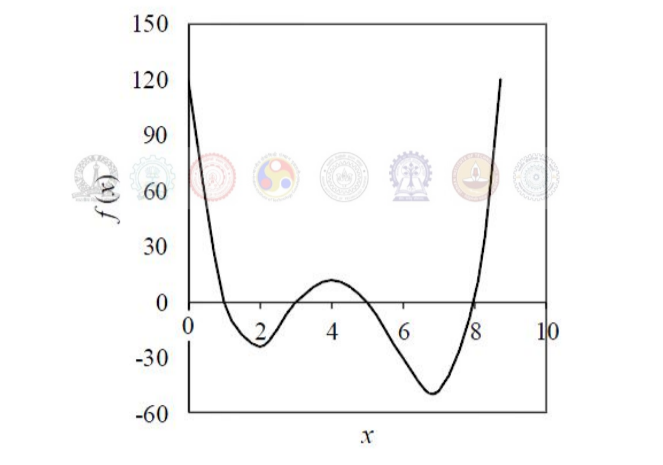
\includegraphics[width = 0.8\columnwidth]{q3.png}
			\caption*{}
			\label{fig:q3}
		\end{figure}
		\hfill{\brak{\text{GATE CH 2017}}}
		
		% Q4 MCQ
		\item Let $\vec{i}$ and $\vec{j}$ be unit vectors in x and y directions respectively. For the function
		\begin{align*}
			F\brak{x,y} = x^3+y^2
		\end{align*}
		the gradient of the function, i.e; $\Delta F$ is given
		\begin{enumerate}
			\begin{multicols}{2}
				\item $3x^2\vec{i} - 2y\vec{j}$
				\item $6x^2y$
				\item $3x^2\vec{i} + 2y\vec{j}$
				\item $2y\vec{i} -3x^2\vec{j}$
			\end{multicols}
		\end{enumerate}
		\hfill{\brak{\text{GATE CH 2017}}}
		
		% Q5 MCQ
		\item The marks obtained by a set of students are: 38, 84. 45, 70, 75, 60. 48.
		
		The mean and median marks, respectively, are
		\begin{enumerate}
			\begin{multicols}{4}
				\item 45 and 75
				\item 55 and 48
				\item 60 and 60
				\item 60 and 70
			\end{multicols}
		\end{enumerate}
		\hfill{\brak{\text{GATE CH 2017}}}
		
		% Q6 MCQ
		\item The volumetric properties of two gases M and N are described by the generalized compressibility chart which expresses the compressibility factor (Z) as a function of reduced pressure and reduced temperature only. The operating pressure P and temperature T of two gases M and N along with  their critical properties \brak{P_{c}, T_{c}} are given in the table below. \\
		\\
		\begin{tabular}{c|c|c|c|c}
			Gas & P\brak{bar} & T\brak{K} & $P_c$\brak{bar} & $T_c$ \\
			\hline
			M & 25 & 300 & 75 & 150 \\
			\hline 
			N & 75 & 1000 & 225 & 500
		\end{tabular} \\
		\\
		$Z_{M}$ and $Z_{N}$ are the compressibility factor of the gases M and N under the given operating conditions. respectively.
		
		The relation between $Z_{M}$ and $Z_{N}$ is
		
		\begin{enumerate}
			\begin{multicols}{4}
				\item $Z_M = 8Z_N$
				\item $Z_M = 3Z_N$
				\item $Z_M = Z_N$
				\item $Z_M = 0.333Z_N$
			\end{multicols}
		\end{enumerate}
		\hfill{\brak{\text{GATE CH 2017}}}
		
		% Q7 MCQ
		\item Water is heated at atmospheric pressure from 40$\degree C$ to 80$\degree C$ using two different processes. In process L. the heating is done by a source at 80$\degree C$. In process II. the water is first heated from 40\degree C to 60\degree C by a source at 60\degree C, and then from 60\degree C to 80\degree C by another source at 80\degree C.
		
		Identify the correct statement.
		\begin{enumerate}
			
				\item Enthalpy change of water in process I is greater than enthalpy change in process II
				\item Enthalpy change of water in process II is greater than enthalpy change in process I
				\item Process I is closer to reversibility
				\item Process II is closer to reversibility
			
		\end{enumerate}
		\hfill{\brak{\text{GATE CH 2017}}}
		
		% Q8 MCQ
		\item In a venturi meter. $\Delta P_1$ and $\Delta P_2$ are the pressure drops corresponding to volumetric flowrates $Q_1$ and $Q_2$. If Q2/Q12. then $\Delta P_2/\Delta P_1$ equals
		\begin{enumerate}
			\begin{multicols}{4}
				\item 2
				\item 4
				\item 0.5
				\item 0.25
			\end{multicols}
		\end{enumerate}
		\hfill{\brak{\text{GATE CH 2017}}}
		
		% Q9 MCQ
		\item The thickness of laminar boundary layer over a flat plate varies along the distance from the leading edge of the plate. As the distance increases, the boundary layer thickness
		\begin{enumerate}
			\begin{multicols}{2}
				\item increases
				\item decreases
				\item initially increases and then decreases
				\item initially decreases and then increases
			\end{multicols}
		\end{enumerate}
		\hfill{\brak{\text{GATE CH 2017}}}
		
		% Q10 MCQ
		\item	Which of the following is the correct sequence of equipment for size reduction of solids?
		\begin{enumerate}
			\begin{multicols}{2}
				\item 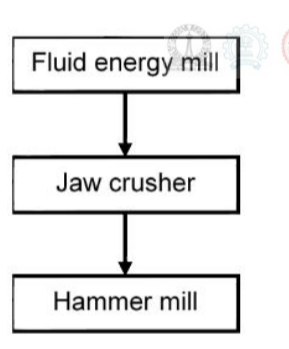
\includegraphics[width = 0.2\columnwidth]{q10a.png}
0				\item 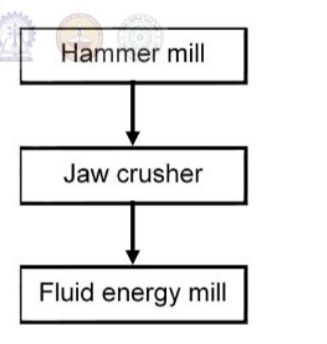
\includegraphics[width = 0.2\columnwidth]{q10b.png}
				\item 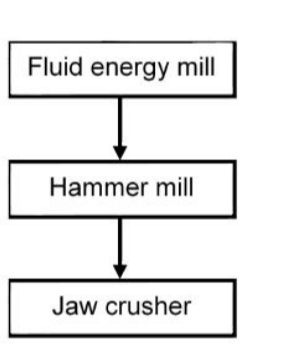
\includegraphics[width = 0.2\columnwidth]{q10c.png}
				\item 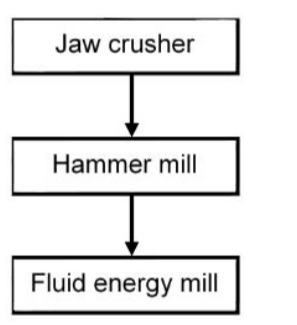
\includegraphics[width = 0.2\columnwidth]{q10d.png}
		    \end{multicols} 	
		\end{enumerate}
		\hfill{\brak{\text{GATE CH 2017}}}
		
		% Q11 NAT
		\item A gas bubble \brak{\text{gas density} \rho_{g} = 2kg/m^3 \text{bubble diameter} D = 10^{-4}m} is rising vertically through water \brak{\text{density} \rho = 1000kg /m^3 \text{viscosity} \mu = 0.001 Pa.s}. Force balance on the bubble leads to the following equation, where v is the velocity of the bubble at any given time t. Assume that the volume of the rising bubble does not change. The value of $g = 9.81m/s^2$ 
			\begin{align*}
				\frac{dv}{dt} = -g\frac{\rho_g-\rho}{\rho_g} - \frac{18\mu}{\rho_g D^2}v
			\end{align*}
			
			The terminal rising velocity of the bubble (in cm/s), rounded to 2 decimal places, is  \underline{\hspace{2cm}} cm/s
			\hfill{\brak{\text{GATE CH 2017}}}
			
			% Q12 MCQ
			\item The one-dimensional unsteady heat conduction equation is
			\begin{align*}
				\rho C_p\frac{\delta T}{\delta t} = \frac{1}{r^n}\frac{\delta}{\delta r}\brak{r^nk\frac{\delta T}{\delta r}}
			\end{align*}
			where T temperature, t-time, r radial position, k thermal conductivity, $\rho$ density, and $C_p$ - specific heat.
			
			For the cylindrical coordinate system, the value of n in the above equation is
			
			\begin{enumerate}
				\begin{multicols}{4}
					\item 0
					\item 1
					\item 2
					\item 3
				\end{multicols}
			\end{enumerate}
			\hfill{\brak{\text{GATE CH 2017}}}
			
			% Q13 NAT
			\item n a heat exchanger, the inner diameter of a tube is 25 mm and its outer diameter is 30 mm. The overall heat transfer coefficient based on the inner area is $360 W/m^2 \degree C$. Then, the overall heat transfer coefficient based on the outer area, rounded to the nearest integer, is  \underline{\hspace{2cm}}  $W/m^2 \degree C$
			
			
			\hfill{\brak{\text{GATE CH 2017}}}
			
			% Q14 MCQ
			\item Which of the following conditions are valid at the plait point?
			\begin{enumerate}[]
				
				
				\item [(P)] Density difference between the extract and raffinate phases is zero
				
				\item[(Q)] Interfacial tension between the extract and raffinate phases is zero
				
				\item[(R)] Composition difference between the extract and raffinate phases is zero
			\end{enumerate}
			\begin{enumerate}
				\begin{multicols}{4}
					\item P and Q only
					\item Q and R only
					\item P and R only
					\item P, Q and R
				\end{multicols}
			\end{enumerate}
			\hfill{\brak{\text{GATE CH 2017}}}
			
			% Q15 NAT
			\item The composition of vapour entering a tray in a distillation column is 0.47. The average composition of the vapour leaving the tray is 0.53. The equilibrium composition of the vapour corresponding to the liquid leaving this tray is 0.52. All the compositions are expressed in mole fraction of the more volatile component.
			
			The Murphree efficiency based on the vapour phase. rounded to the nearest integer, is  \underline{\hspace{2cm}}  \%.
			\hfill{\brak{\text{GATE CH 2017}}}
			
			% Q16 MCQ
			\item Consider steady state mass transfer of a solute A from a gas phase to a liquid phase. The gas phase bulk and interface mole fractions are $y_{A,G}$ and $y_{A,i}$, respectively. The liquid phase bulk and interface mole fractions are $X_{A,L}$ and $X_{A,i}$ respectively. The ratio $\frac{X_{A,i}-X_{A,L}}{Y_{A,G}-Y_{A,i}}$ is very close to zero. 
			
			This implies that mass transfer resistance is
			\begin{enumerate}
				\begin{multicols}{2}
					\item negligible in gas phase only
					\item negligible in liquid phase only
					\item negligible in both the phases
					\item considerable in both the phases
				\end{multicols}
			\end{enumerate}
			\hfill{\brak{\text{GATE CH 2017}}}
			
			% Q17 MCQ
			\item The following reaction rate curve is shown for a reaction A P. Here, \brak{-r_A} and X represent reaction rate and conversion, respectively. The feed is pure A and 90\% conversion is desired
			\begin{figure}[H]
				\centering
				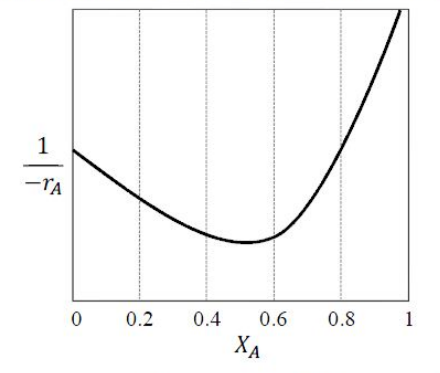
\includegraphics[width = 0.8\columnwidth]{q17.png}
				\caption*{}
				\label{fig:q17}
			\end{figure}
			Which amongst the following reactor configurations gives the lowest total volume of the reactor(s)?
			
			\begin{enumerate}
				\begin{multicols}{2}
					\item CSTR followed by PFR
					\item Two CSTRs in series
					\item PFR followed by CSTR
					\item A single PFR
				\end{multicols}
			\end{enumerate}
			\hfill{\brak{\text{GATE CH 2017}}}
			
			% Q18 MCQ
			\item  Consider a first order catalytic reaction in a porous catalyst pellet.
			
			Given R characteristic length of the pellet: $D_{e}$ effective diffusivity: ke mass transfer coefficient: $k_{1}$ rate constant based on volume of the catalyst pellet; $C_{s}$ concentration of reactant on the pellet surface.
			
			The expression for Thiele modulus is
			\begin{enumerate}
				\begin{multicols}{4}
					\item $\frac{k_C R}{D_e}$
					\item $R\sqrt{\frac{k_1}{D_e}}$
					\item $R\sqrt{\frac{k_1 C_s}{D_e}}$
					\item $R\sqrt{\frac{D_e}{k_1}}$
				\end{multicols}
			\end{enumerate}
			\hfill{\brak{\text{GATE CH 2017}}}
			
			% Q19 MCQ
			\item For a solid-catalyzed gas phase reversible reaction, which of the following statements is ALWAYS TRUE?
			\begin{enumerate}
				
					\item Adsorption is rate limiting
					\item Desorption is rate limiting
					\item Solid catalyst does not affect equilibrium conversion
					\item Temperature doesn't affect equilibrium conversion
				
			\end{enumerate}
			\hfill{\brak{\text{GATE CH 2017}}}
			
			% Q20 MCQ
			\item Match the variables in Group-1 with the instruments in Group-2 \\
			\begin{tabular}{c|c}
				Group-1 & Group 2 \\
				P) Temperature & I) Capacitance probe \\
				Q)Liquid level & II) McLeod gauge \\
				R)Vacuum & III) Chromatograph \\
				S)Concentration & IV) Thermistor
			\end{tabular}
			\begin{enumerate}
				\begin{multicols}{4}
					\item P-IV,Q-III,R-II,S-I
					\item P-I,Q-II,R-IV,S-III
					\item P-IV,Q-I,R-II,S-III
					\item P-III,Q-II,R-I,S-IV
				\end{multicols}
			\end{enumerate}
			\hfill{\brak{\text{GATE CH 2017}}}
			
			% Q21 MCQ
			\item An LVDT (Linear Variable Differential Transformer) is a transducer used for converting
			\begin{enumerate}
				\begin{multicols}{2}
					\item displacement to voltage
					\item voltage to displacement
					\item resistance to voltage
					\item voltage to current
				\end{multicols}
			\end{enumerate}
			\hfill{\brak{\text{GATE CH 2017}}}
			
			% Q22 NAT
			\item The cost of a new pump (including installation) is 24,000 Rupees. The pump has a useful life of 10 years. Its salvage value is 4000 Rupees. Assuming straight line depreciation, the book value of the pump at the end of 4th year. rounded to the nearest integer is  \underline{\hspace{2cm}}  Rupees.
			\hfill{\brak{\text{GATE CH 2017}}}
			
			% Q23 MCQ
			\item The DCDA (Double Contact Double Absorption) process is used for the manufacture of
			\begin{enumerate}
				\begin{multicols}{4}
					\item urea
					\item sulphuric acid
					\item nitric acid
					\item ammonia
				\end{multicols}
			\end{enumerate}
			\hfill{\brak{\text{GATE CH 2017}}}
			
			% Q24 MCQ
			\item Match the polymerization processes in Group-1 with the polymers in Group-2. \\
			\begin{tabular}{ c c }
				Group-1 & Group-2 \\
				P)Free radical polymerisation & I)Nylon 6,6 \\
				Q)Ziegler-natta polymerisation & II)Polypropylene\\
				R)Condensation polymerisation & III) PVC
			\end{tabular}
			\begin{enumerate}
				\begin{multicols}{2}
					\item P-I, Q-II, R- III
					\item P-III, Q-II, R- I
					\item P-I, Q-III, R- II
					\item P-II, Q-I, R- III
				\end{multicols}
			\end{enumerate}
			\hfill{\brak{\text{GATE CH 2017}}}
			
			% Q25 MCQ
			\item The purpose of methanation reaction used in ammonia plants is to
			\begin{enumerate}
				\begin{multicols}{1}
					\item remove CO as it is a catalyst poison
					\item increase the amount of hydrogen
					\item remove sulphur as it is a catalyst poison
					\item utilize methane as a catalyst for ammonia synthesis
				\end{multicols}
			\end{enumerate}
			\hfill{\brak{\text{GATE CH 2017}}}
			
		
			% Q26 NAT
			\item For the initial value problem 
			\begin{align*}
				\frac{dx}{dt} = sin\brak{t}, x\brak{0}=0
			\end{align*}
			the value of x at $t = \pi/3$ is  \underline{\hspace{2cm}} 
			\hfill{\brak{\text{GATE CH 2017}}}
			
			% Q27 MCQ
			\item The Laplace transform of a function is $\frac{s+1}{s(s+2)}$ The initial and final values, respectively, of the function are
			\begin{enumerate}
				\begin{multicols}{2}
					\item 0 and 1
					\item 1 and 1/2
					\item 1/2 and 1
					\item 1/2 and 0
				\end{multicols}
			\end{enumerate}
			\hfill{\brak{\text{GATE CH 2017}}}
			
			% Q28 MCQ
			\item Match the problem type in Group-1 with the numerical method in Group-2. \\
			\begin{tabular}{c|c}
				Group 1 & Group 2 \\
				P)System of linear algebraic equations & I0 Newton-Raphson \\
				Q) Non-linear algebraic equations & II)Gauss-Seidel \\
				R)Ordinary differential equations & III)Simpson's rule \\
				S)Numerical integration & IV) Runge-Kutta
			\end{tabular}
				
			\begin{enumerate}
				\begin{multicols}{2}
					\item  P-II, Q-I, R-III, S-IV
					\item  P-I, Q-II, R-IV, S-III
					\item  P-IV, Q-III, R-II, S-I
					\item  P-II, Q-I, R-IV, S-III
				\end{multicols}
			\end{enumerate}
			\hfill{\brak{\text{GATE CH 2017}}}
			
			% Q29 NAT
			\item  A box has 6 red balls and 4 white balls. A ball is picked at random and replaced in the box, after which a second ball is picked.
			The probability of both the balls being red, rounded to 2 decimal places, is  \underline{\hspace{2cm}} 
			\hfill{\brak{\text{GATE CH 2017}}}
			
			% Q30 NAT
			\item An aqueous salt-solution enters a crystallizer operating at steady state at 25$\degree C$. The feed temperature is 90$\degree C$ and the salt concentration in the feed is 40 weight \%. The salt crystallizes as a pentahydrate. The crystals and the mother liquor leave the crystallizer. The molecular weight of the anhydrous salt is 135. The solubility of the salt at 25$\degree C$ is 20 weight \%.
			
			The feed flowrate required for a production rate of 100 kg/s of the hydrated salt, rounded to the nearest integer. is kg/s
			\hfill{\brak{\text{GATE CH 2017}}}
			
			% Q31 NAT
			\item Reaction $A\rightarrow B$ is carried out in a reactor operating at steady state and 1 mol/s of pure A at $425\degree C$ enters the reactor. The outlet stream leaves the reactor at $325 \degree C$. The heat input to the reactor is 17 kW. The heat of reaction at the reference temperature of $25\degree C $is 30 kJ/mol. The specific heat capacities (in kJ/mol.K) of A and B are 0.1 and 0.15. respectively.
			
			The molar flowrate of B leaving the reactor, rounded to 2 decimal places, is  \underline{\hspace{2cm}}  mol/s
			\hfill{\brak{\text{GATE CH 2017}}}
			
			% Q32 NAT
			\item The pressure of a liquid is increased isothermally. The molar volume of the liquid decreases from $50.45- 106 m^3/mol$ to $48�10 m^3/mol$ during this process. The isothermal compressibility of the liquid is 10 Pa, which can be assumed to be independent of pressure.
			The change in the molar Gibbs free energy of the liquid, rounded to nearest integer is  \underline{\hspace{2cm}}  J/mol
			\hfill{\brak{\text{GATE CH 2017}}}
			
			% Q33 NAT
			\item A sparingly soluble gas (solute) is in equilibrium with a solvent at 10 bar. The mole fraction of the solvent in the gas phase is 0.01. At the operating temperature and pressure, the fugacity coefficient of the solute in the gas phase and the Henry's law constant are 0.92 and 1000 bar, respectively. Assume that the liquid phase obeys Henry's law.
			The MOLE PERCENTAGE of the solute in the liquid phase, rounded to 2 decimal places, is  \underline{\hspace{2cm}} 
			\hfill{\brak{\text{GATE CH 2017}}}
			
			% Q34 NAT
			\item The vapour pressure of a pure substance at a temperature 7 is 30 bar. The actual and ideal gas values of g/RT for the saturated vapour at this temperature 7 and 30 bar are 7.0 and 7.7. respectively. Here. g is the molar Gibbs free energy and R is the universal gas constant.
			
			The fugacity of the saturated liquid at these conditions, rounded to 1 decimal place, is  \underline{\hspace{2cm}} 
			\hfill{\brak{\text{GATE CH 2017}}}
			
			% Q35 NAT
			\item Oil is being delivered at a steady flowrate through a circular pipe of radius $1.25�10^-2$ m and length 10 m. The pressure drop across the pipe is 500 Pa.
			
			The shear stress at the pipe wall, rounded to 2 decimal places, is  \underline{\hspace{2cm}}  Pa.
			
			% Q36 MCQ
			\item  The following table provides four sets of Fanning friction factor data, for different values of Reynolds number (Re) and roughness factor (k/D)\\
			
			\begin{tabular}{ c c c c c c }
				 & Re & $10^2$ & $10^3$ & $10^5$ & $10^6$\\
			\hline
				 & \brak{\frac{k}{D}} & 0 & 0.001 & 0 & 0.001 \\
			\hline
			Set I & f &	  0.16 & 0.016 & $16\times10^{-5}$ & $16\times10^{-5}$ \\
			Set II & f & 0.016 & 0.16 & 0.0055 & 0.0045 \\
			Set III & f & 0.16 & 0.016 & 0.0045 & 0.0055 \\
			Set IV & f & 0.0045 & 0.0055 & 0.016 & 0.16 \\
			\hline
			\end{tabular} \\
			Which of the above sets of friction factor data is correct?
			\hfill{\brak{\text{GATE CH 2017}}}
			\begin{enumerate}
				\begin{multicols}{4}
					\item Set I
					\item Set II
					\item Set III
					\item Set IV
				\end{multicols}
			\end{enumerate}
			\hfill{\brak{\text{GATE CH 2017}}}
			
			% Q37 NAT
			\item A propeller \brak{\text{diameter D = 15 m}} rotates at N = 1 revolution per second (rps). To understand the flow around the propeller. a lab-scale model is made. Important parameters to study the flow are velocity of the propeller tip \brak{V = \pi ND}, diameter D and acceleration due to gravity (g). The lab-scale model is 1/100th of the size of the actual propeller.
			
			The rotation speed of the lab-scale model, to the nearest integer, should be  \underline{\hspace{2cm}}  rps
			\hfill{\brak{\text{GATE CH 2017}}}
			
			% Q38 NAT
			\item Size analysis was carried out on a sample of gravel. The data for mass fraction $\chi_1$ and average particle diameter $D_{pi}$ of the fraction is given in the table below:\\
			\begin{tabular}{ c c }
				$x_i$ & $D_{pi}$ \\
				\hline
				0.2 & 5 \\
				0.4 & 10 \\
				0.4 & 20 \\
				\hline
			\end{tabular}
			
			 
			The mass mean diameter of the sample. to the nearest integer, is  \underline{\hspace{2cm}} 
			\hfill{\brak{\text{GATE CH 2017}}}
			
			% Q39 MCQ
			\item Let $I_{b\lambda}$ be the spectral blackbody radiation intensity per unit wavelength about the wavelength $\lambda$. The blackbody radiation intensity emitted by a blackbody over all wavelengths is
			\begin{enumerate}
				\begin{multicols}{4}
					\item $\frac{dI_{b\lambda}}{d\lambda}$
					\item $\frac{d^2I_{b\lambda}}{d\lambda^2}$
					\item $\int_{0}^{\infty} I_{b\lambda} d\lambda$
					\item $\int_{0}^{\infty} \lambda I_{b\lambda} d\lambda$
				\end{multicols}
			\end{enumerate}
			\hfill{\brak{\text{GATE CH 2017}}}
			
			% Q40 MCQ
			\item A fluid flows over a heated horizontal plate maintained at temperature $T_{w}$ The bulk temperature of the fluid is $T_\infty$ The temperature profile in the thermal boundary layer is given by:
			\begin{align*}
				T = T_w + \brak{T_w - T_\infty}\sbrak{\frac{1}{2}\frac{y}{\delta_t}^3 - \frac{3}{2}\frac{y}{\delta_t}}			\end{align*}
			Here. y is the vertical distance from the plate, $\delta_{t}$ is the thickness of the thermal boundary layer and k is the thermal conductivity of the fluid.
			
			The local heat transfer coefficient is given by
			\begin{enumerate}
				\begin{multicols}{4}
					\item $\frac{k}{2\delta_t}$
					\item $\frac{k}{\delta_t}$
					\item $\frac{3k}{2\delta_t}$
					\item $\frac{2k}{\delta_t}$
				\end{multicols}
			\end{enumerate}
			\hfill{\brak{\text{GATE CH 2017}}}
			
			% Q41 MCQ
			\item In nucleate boiling. the pressure inside a bubble is higher than the pressure of the surrounding liquid. Assuming that both the liquid and vapour are saturated, the temperature of the liquid will ALWAYS be
			\begin{enumerate}
				\begin{multicols}{2}
					\item at $100 \degree C$
					\item lower than temperature of vapour
					\item equal to temperature of vapour
					\item higher than temperature of vapour
				\end{multicols}
			\end{enumerate}
			\hfill{\brak{\text{GATE CH 2017}}}
			
			% Q42 NAT
			\item The vapor phase composition and relative volatilities (with respect to n-propane) on an ideal tray of a distillation column are\\
			\\
			\begin{tabular}{c|c|c|c}
				Component & Methane & Ethane & n-Propane \\
				Mole fraction in vapour & 0.12 & 0.28 & 0.60 \\
				Relative volatility & 10 & 4 & 1
			\end{tabular}\\
			\\
			The mole fraction of n-propane in the liquid phase, rounded to 2 decimal places, is  \underline{\hspace{2cm}} 
			
			\hfill{\brak{\text{GATE CH 2017}}}
			
			% Q43 MCQ
			\item The Sherwood number $S*h_{L}$ correlation for laminar flow over a flat plate of length L is given 
			\begin{align*}		
			Sh_{L} = 0.664Re_{L}^{0.5} Sc^(1/3) 
		 \end{align*}
			where $Re_{L}$ and Sc represent Reynolds number and Schmidt number, respectively.
			
			This correlation, expressed in the form of Chilton-Colburn $j_{D}$ factor. is
			\begin{enumerate}
				\begin{multicols}{4}
					\item $j_{D} = 0.664$
					\item $j_{D} = 0.664 Re_{L}^{-0.5}$
					\item $j_{D} = 0.664Re_{L}$
					\item $j_{D} = 0.664Re_{L}^{0.5}Sc^{2/3}$
				\end{multicols}
			\end{enumerate}
			\hfill{\brak{\text{GATE CH 2017}}}
			
			% Q44 NAT
			\item In a countercurrent stripping operation using pure steam, the mole ratio of a solute in the liquid stream is reduced from 0.25 to 0.05. The liquid feed flowrate, on a solute-free basis, is 3 mol/s. The equilibrium line for the system is given in the figure below.
			\begin{figure}[H]
				\centering
				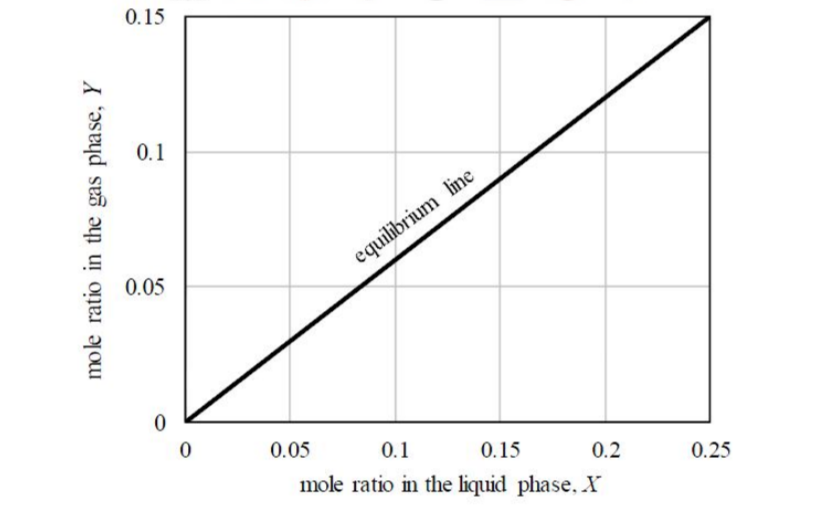
\includegraphics[width = 0.8\columnwidth]{q44.png}
				\caption*{}
				\label{fig:44}
			\end{figure}
			
			
			The MINIMUM flowrate of pure steam for this process, rounded to 1 decimal place, is   \underline{\hspace{2cm}}  mol/s 
			\hfill{\brak{\text{GATE CH 2017}}}
			
			% Q45 NAT
			\item In a batch adsorption process. 5 g of fresh adsorbent is used to treat 1 liter of an aqueous phenol solution. The initial phenol concentration is 100 mg/liter. The equilibrium relation is given by
			\begin{align*}
			q = 1.3C
			\end{align*}
			where q' is the amount of phenol adsorbed in mg of phenol per gram of adsorbent, and C is the concentration of phenol in mg/liter in the aqueous solution.
			
			When equilibrium is attained between the adsorbent and the solution, the concentration of phenol in the solution, rounded to 1 decimal place, is  \underline{\hspace{2cm}}  mg/liter.
			\hfill{\brak{\text{GATE CH 2017}}}
			
			% Q46 NAT
			\item The C-curve measured during a pulse tracer experiment is shown below. In the figure, C(t) is the concentration of the tracer measured at the reactor exit in mol/liter at time t seconds
			\begin{figure}[H]
				\centering
				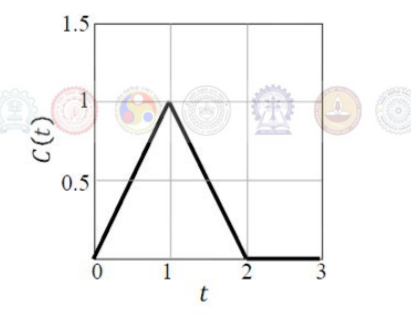
\includegraphics[width = 0.8\columnwidth]{q46.png}
				\caption*{}
				\label{fig:46}
			\end{figure}
			The mean residence time in the reactor, rounded to 1 decimal place, is  \underline{\hspace{2cm}}  S
			\hfill{\brak{\text{GATE CH 2017}}}
			
			% Q47 NAT
			\item The following liquid phase second-order reaction is carried out in an isothermal CSTR at steady state
			\begin{align*}
			 A\rightarrow R, -r_a=0.00502C_A^{2} mol/m^3.hr
			\end{align*}
			where $C_A$ is the concentration of the reactant in the CSTR. The reactor volume is $2 m^3$, the inlet flowrate is $0.5 m^3/hr$ and the inlet concentration of the reactant is 1000 mol/m
			The fractional conversion, rounded to 2 decimal places is  \underline{\hspace{2cm}} 
			\hfill{\brak{\text{GATE CH 2017}}}
			
			% Q48 NAT
			\item The reversible reaction of t-butyl alcohol (TBA) and ethanol (EtOH) to ethyl t-butyl ether (ETBE) is
			\begin{align*}
				TBA + EtOH \leftrightharpoons ETBE + Water
			\end{align*}
			The equilibrium constant for this reaction is Kc = 1. Initially. 74 g of TBA is mixed with 100 g of aqueous solution containing 46 weight\% ethanol. The molecular weights are: 74 g/mol for TBA, 46 g/mol for EtOH. 102 g/mol for ETBE. and 18 g/mol for water.
			The mass of ETBE at equilibrium, rounded to 1 decimal place, is  \underline{\hspace{2cm}} 
			\hfill{\brak{\text{GATE CH 2017}}}
			
			% Q49 NAT
			\item The following gas-phase reaction is carried out in a constant-volume isothermal batch reactor
			\begin{align*}
			A+B \rightarrow R+S
		    \end{align*}
			
			The reactants A and B as well as the product S are non-condensable gases. At the operating temperature, the saturation pressure of the product R is 40 kPa.
			
			Initially, the batch reactor contains equimolar amounts of A and B (and no products) at a total pressure of 100 kPa. The initial concentrations of the reactants are $C_{A,0} = ?_{B,0} = 12.5 mol/m^3$. The rate of reaction is given by $-r_A = 0.08 C_AC_B mol/m^3.s.$
			
			
			The time at which R just starts condensing, rounded to 1 decimal place, is  \underline{\hspace{2cm}} 
			\hfill{\brak{\text{GATE CH 2017}}}
			
			% Q50 NAT
			\item The transfer function of a system is
			\begin{align*}
			\frac{1}{4s^2+1.2s+1}
		\end{align*}
			For a unit step increase in the input, the fractional overshoot, rounded to 2 decimal places. is  \underline{\hspace{2cm}} 
			\hfill{\brak{\text{GATE CH 2017}}}  
			
			% Q51 NAT
			\item The open loop transfer function of a process with a proportional controller (gain Kc) is
			\begin{align*}
			G_OL =  K_c \frac{e^{-2s}}{s}
			\end{align*}
			Based on the Bode criterion for closed-loop stability, the ultimate gain of the controller, rounded to 2 decimal places, is  \underline{\hspace{2cm}} 
			\hfill{\brak{\text{GATE CH 2017}}}
			
			% Q52 NAT
			\item The characteristic equation of a closed-loop system is
			\begin{align*}
			6s^3+11s^2+6s+1+K = 0, where K > 0
			\end{align*}
			The value of K beyond which the system just becomes unstable, rounded to the nearest integer is  \underline{\hspace{2cm}} 
			\hfill{\brak{\text{GATE CH 2017}}}
			
			% Q53 NAT
			\item A bond has a maturity value of 20.000 Rupees at the end of 4 years. The interest is compounded at the rate of 5\% per year
			
			The initial investment to be made, rounded to the nearest integer, is  \underline{\hspace{2cm}} Rupees
			\hfill{\brak{\text{GATE CH 2017}}}
			
			% Q54 NAT
			\item The total cost $C_T$ of an equipment in terms of the operating variables x and y is 
			\begin{align*}
        C_T = 2x +  \frac{12000}{xy} + y + 5
    \end{align*}
			
			The optimal value of $C_T$ rounded to 1 decimal place,  \underline{\hspace{2cm}} 
			\hfill{\brak{\text{GATE CH 2017}}}
			
			% Q55 MCQ
			\item Match the equipment in Group-1 with the process in Group-2
			\begin{tabular}{c|c}
				Group-1 & Group-2 \\
				P) Fluidized bed & I) Paper-making \\
				Q) Multistage adiabatic reactor with inter-stage cooling & II) Sodium hydroxide manufacture \\
				R) Fourdrinier machine & III)SO2 oxidation \\
				S) Diaphragm cell & IV) Catalytic cracking
			\end{tabular}
			\begin{enumerate}
				\begin{multicols}{2}
					\item P-IV, Q-III, R-I, S-II
					\item P-IV, Q-III, R-II, S-I
					\item P-III, Q-IV, R-I, S-II
					\item P-III, Q-IV, R-II, S-I
				\end{multicols}
			\end{enumerate}
			\hfill{\brak{\text{GATE CH 2017}}}
			
			% Q56 MCQ
			\item The bacteria in milk are destroyed when it heated to 80 degree Celsius.
			\begin{enumerate}
				\begin{multicols}{4}
					\item would be
					\item will be
					\item is
					\item was
				\end{multicols}
			\end{enumerate}
			\hfill{\brak{\text{GATE CH 2017}}}
			
			% Q57 MCQ
			\item with someone else's email account is now a very serious offence.
			\begin{enumerate}
				\begin{multicols}{4}
					\item Involving
					\item Assisting
					\item Tampering
					\item Incubating
				\end{multicols}
			\end{enumerate}
			\hfill{\brak{\text{GATE CH 2017}}}
			
			% Q58 MCQ
			\item Consider the following sentences:
			
			All benches are beds. No bed is a bulb. Some bulbs are lamps.
			
			Which of the following can be inferred?
			\begin{enumerate}[]
				 
			
			\item[i.] Some beds are lamps.
			
			\item[ii.] Some lamps are beds.
		\end{enumerate}
			\begin{enumerate}
				\begin{multicols}{4}
					\item Only i
					\item Only ii
					\item Both i and ii
					\item Neither i nor ii
				\end{multicols}
			\end{enumerate}
			\hfill{\brak{\text{GATE CH 2017}}}
			
			% Q59 MCQ
			\item If the radius of a right circular cone is increased by 50\%. its volume increases by
			\begin{enumerate}
				\begin{multicols}{4}
					\item 75\%
					\item 100\%
					\item 125\%
					\item 237.5\%
				\end{multicols}
			\end{enumerate}
			\hfill{\brak{\text{GATE CH 2017}}}
			
			% Q60 MCQ
			\item The following sequence of numbers is arranged in increasing order: 1, x, x, x, y, y, 9,16,18. Given that the mean and median are equal. and are also equal to twice the mode the value of y is
			\begin{enumerate}
				\begin{multicols}{4}
					\item 5
					\item 6
					\item 7
					\item 8
				\end{multicols}
			\end{enumerate}
			\hfill{\brak{\text{GATE CH 2017}}}
			
			% Q61 MCQ
			\item The old concert hall was demolished because of fears that the foundation would be affected by the construction of the new metro line in the area. Modern technology for underground metro construction tried to mitigate the impact of pressurized air pockets created by the excavation of large amounts of soil. But even with these safeguards. it was feared that the soil below the concert hall would not be stable.
			From this one can infer that
			\begin{enumerate}
				\begin{multicols}{1}
					\item the foundations of old buildings create pressurized air pockets underground, which are difficult to handle during metro construction
					\item metro construction has to be done carefully considering its impact on the foundations of existing buildings
					\item old buildings in an area form an impossible hurdle to metro construction in that area
					\item pressurized air can be used to excavate large amounts of soil from underground areas.
				\end{multicols}
			\end{enumerate}
			\hfill{\brak{\text{GATE CH 2017}}}
			
			% Q62 MCQ
			\item  Students applying for hostel rooms are allotted rooms in order of seniority. Students already staying in a room will move if they get a room in their preferred list. Preferences of lower ranked applicants are ignored during allocation.
			Given the data below. which room will Ajit stay in?
			\begin{table}[h!]
				\centering\begin{tabular}{c|c|c|c}
				\hline
				\textbf{Names} & \textbf{Student seniority} & \textbf{Current room} & \textbf{Room preference list} \\
				\hline
				Amar & 1 & P & R,S,Q \\
				\hline
				Akbar & 2 & None & R, S \\
				\hline
				Anthony & 3 & Q & P \\
				\hline
				Ajit & 4 & 5 & Q,P,R \\
			\end{tabular}
			\end{table}
			\begin{enumerate}
				\begin{multicols}{4}
					\item P
					\item Q
					\item R
					\item S
				\end{multicols}
			\end{enumerate}
			\hfill{\brak{\text{GATE CH 2017}}}
			
			% Q63 MCQ
			\item The last digit of $2171^7 + 2172^9 + 2173^{11} + 2174^{13}$ is
			\begin{enumerate}
				\begin{multicols}{4}
					\item 2
					\item 4
					\item 6
					\item 8
				\end{multicols}
			\end{enumerate}
			\hfill{\brak{\text{GATE CH 2017}}}
			
			% Q64 MCQ
			\item Two machines M1 and M2 are able to execute any of four jobs P. Q. R and S. The machines can perform one job on one object at a time. Jobs P. Q. R and S take 30 minutes. 20 minutes. 60 minutes and 15 minutes each respectively. There are 10 objects each requiring exactly 1 job. Job P is to be performed on 2 objects. Job Q on 3 objects. Job R on 1 object and Job S on 4 objects. What is the minimum time needed to complete all the jobs?
			\begin{enumerate}
				\begin{multicols}{4}
					\item 2 hours
					\item 2.5 hours
					\item 3 hours
					\item 3.5 hours
				\end{multicols}
			\end{enumerate}
			\hfill{\brak{\text{GATE CH 2017}}}
			
			% Q65 MCQ
			\item The bar graph below shows the output of five carpenters over one month. each of whom made different items of furniture: chairs, tables. and beds.
			\begin{figure}[H]
				\centering
				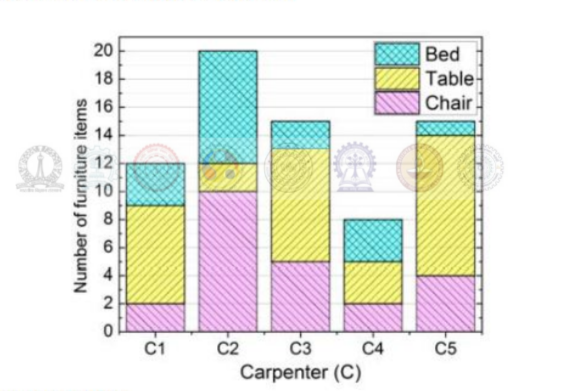
\includegraphics[width = 0.8\columnwidth]{q65.png}
				\caption*{}
				\label{fig:q65}
			\end{figure}
			
			Consider the following statements.
			\begin{enumerate}[]
				
			
		\item [i.] The mumber of beds made by carpenter C2 is exactly the same as the number of tables made by carpenter C3.
			
		\item[ii.] The total number of chairs made by all carpenters is less than the total number of tables.
		\end{enumerate}
			Which one of the following is true?
			\begin{enumerate}
				\begin{multicols}{4}
					\item Only i
					\item Only ii
					\item Both i and ii
					\item Neither i nor ii
				\end{multicols}
			\end{enumerate}
			\hfill{\brak{\text{GATE CH 2017}}}
		
		\end{enumerate}
		
	\end{document}